
\begin{figure}
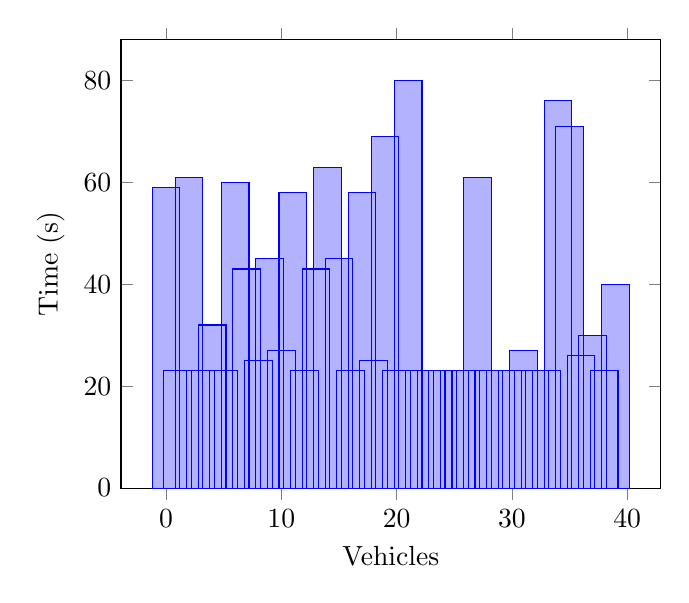
\begin{tikzpicture}
\begin{axis}[
legend style={anchor=west},
xlabel=Vehicles,
ylabel=Time (s),
ymin=0,
ybar,
]
\addplot coordinates {
(0, 59)
(1, 23)
(2, 61)
(3, 23)
(4, 32)
(5, 23)
(6, 60)
(7, 43)
(8, 25)
(9, 45)
(10, 27)
(11, 58)
(12, 23)
(13, 43)
(14, 63)
(15, 45)
(16, 23)
(17, 58)
(18, 25)
(19, 69)
(20, 23)
(21, 80)
(22, 23)
(23, 23)
(24, 23)
(25, 23)
(26, 23)
(27, 61)
(28, 23)
(29, 23)
(30, 23)
(31, 27)
(32, 23)
(33, 23)
(34, 76)
(35, 71)
(36, 26)
(37, 30)
(38, 23)
(39, 40)
};

\end{axis}
\end{tikzpicture}
\label{tik:100:3_V, 3_V.-60, 2_V}
\caption{100 percent diving with GSC on route $3_V, 3_V.-60, 2_V$}
\end{figure}
